% !TeX encoding = UTF-8

\chapter{REVISÃO BIBLIOGRÁFICA}\label{ch:rev-bibs}

Vários trabalhos serviram como fonte de conhecimento e suporte para o entendimento e desenvolvimento deste tema. Alguns foram considerados mais importantes por abordar detalhadamente o problema de reconhecimento, outros foram buscados para se entender melhor, ou ter outra visão sobre algum detalhes específico do problema.

Trabalhos de autores como \cite{geysilva} ajudaram a estruturar e organizar o tema por abordar tópicos similares e por possuir riqueza de detalhes no assunto de análise de componentes apresentando uma implementação em \textit{MatLab} (um \textit{software} interativo voltado para o cálculo numérico).

O trabalho de \cite{img-digital-willians} foi utilizado para se aprofundar no tema de imagens digitais, assim como  \cite{gonzalez_woods} que também esclareceu o funcionamento de escalonamento, normalização e mono cromatização de imagens. O autor Dr. Andrew Davison em seus trabalhos, dentre os quais, \cite{drmathew_java_programming} se destacou pela ótima didática facilitando o entendimento de Análise de Componentes e sua relação com \textit{EigenFaces}, disponibilizando ainda exemplos de implementação em \textit{JAVA}. 

Os trabalhos \cite{tutorial_en_smith} e \cite{tutorial_pt} foram estudados como tutoriais do processo de ACP e será usado posteriormente como guias de implementação do algorítimo.

Nas próximas seções serão explanados os conteúdos destes e de outros trabalhos disponibilizados em uma ordem didática.


\section{AQUISIÇÃO E PROCESSAMENTO DE IMAGENS E VÍDEO}\label{sec:processamento_imagens}

Com a abrangência dos sistemas de comunicação, com difusão de conhecimentos informações pelos diversos meios, captar, armazenar e processar imagens se tornou necessidade fundamental. Para o reconhecimento de faces em vídeo, o sucesso deste processo é pré-requisito  para o funcionamento dos algoritmos. 

As sessões a seguir contemplam fundamentos básicos sobre imagem, vídeo, a alguns de seus processamentos necessários para a aplicação dos algoritmos de detecção e reconhecimento de faces.


\subsection{IMAGEM E VÍDEO DIGITAL}\label{subsec:imagem}

A imagem digital são valores numéricos disponibilizados em uma matriz bidimensional. Basicamente existem dois tipos de imagens: os chamados \textit{rasters} ou \textit{bitmaps}, e vetorizadas. A primeira são representações de cada ponto da imagem com alguma cor usadas geralmente em fotografias, enquanto que o segundo é produzido por plotadores que recebem os pontos e as distâncias entre eles como parâmetros, consideranto retas, curvas, polígonoas e etc, sendo assim não perdem sua qualidade quando redimensionados.

Converter uma imagem para o formato digital significa transferir os elementos que a compõem para elementos representativos de cada pequeno fragmento original. O menor elemento da imagem, o \textit{pixel}, é identificado segundo sua intensidade de nível de cinza e as cores correspondentes. Identificados, estes elementos são armazenados por códigos que podem ser reconhecidos pelo dispositivo de visualização e apresentados novamente por um dispositivo de visualização, como um monitor de vídeo ou impressora \cite{img-digital-willians}. 

%\vspace*{13cm}
\begin{figure}[h]
	\centering
	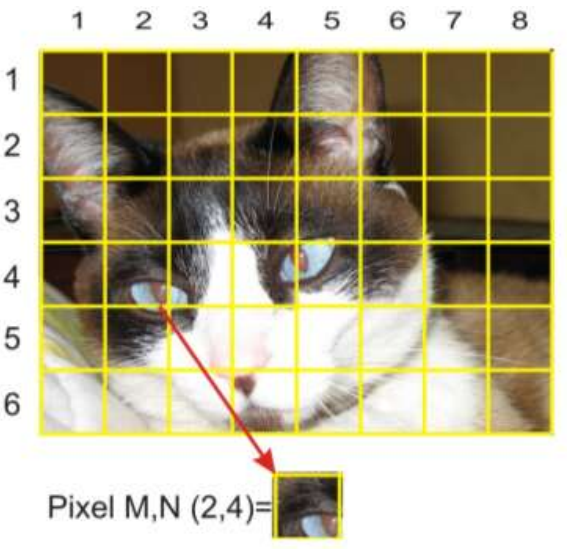
\includegraphics[width=.6\textwidth]{pixel-img}
	\caption{Exemplo de imagem representada como uma matriz (M,N) de pixels, com destaque para o pixel (2,4).}
	\fonte{\cite{img-digital-willians}}
	\label{pixel_img}
\end{figure}



Uma imagem analógica que é a (representação real da cena, para ser convertida para o formato do
processamento computacional deve sofrer uma separação espacial (amostragem) e em amplitude
(quantização) \cite{img-digital-willians}. 

A amostragem é a divisão do plano x,y em uma grade (ou matriz bi dimensional) onde x e y serão números inteiros. Os pontos da matriz de são denominados \textit{pixels} (\textit{PICTure Elements}), como ilustra a \autoref{pixel_img}. Cada pixel representa uma parte da cena real, desta forma a resolução espacial da imagem é proporcional aos valores de M e N correspondentes na matriz (exemplo Fig.22). Em geral a malha de amostragem, o formato dos pixels (x,y), é retangular, mas pode também ser triangular ou mais complexa. Os valores de cada ponto da matriz, coluna x linha (xy), que identifica um único pixel (M,N0, devem ser escolhidos de forma a respeitar a relação qualidade da imagem x espaço de armazenamento, em função da aplicação para a qual a imagem se destina. Para uma imagem digital com 256 níveis de cinza o número de bytes ocupados para armazenar a imagem é o produto da linha vezes a coluna da matriz \cite{img-digital-willians}. 

Matematicamente, toda imagem monocromática (preto e branco) é um função f(x,y) da intensidade luminosa, em qualquer parte das coordenadas (x,y), proporcional ao brilho (tons de cinza) da imagem em um determinado ponto. A figura mostra uma imagem e como representamos os eixos x e y no plano cartesiano \cite{gonzalez_woods}. 

A função  f(x,y)  é a multiplicação da iluminância  i(x,y) (que é a quantidade de luz que incide sobre o objeto) pela refletância  r(x,y)  (que é fração de luz incidente que o objeto vai refletir ao ponto (x,y). 

Sendo assim, podemos dizer que \cite{gonzalez_woods}:

f(x,y) = i(x,y) * r(x,y),

onde 0 < i(x,y) e 0 < r(x,y) < 1 .



\subsection{FORMATO PNG}\label{subsec:png}

O PNG (\textit{Portable Network Graphics} ou "\textit{PNG is Not Giff}") é um formato de representação de imagens do tipo \textit{rasters}. foi desenhado para substituir o formato GIF e o TIFF em certa extensão. O PNG tem 3 vantagens principais: suporta canal alfa (transparência) de forma eficiente, tem a maior gama de profundidade de cores e alta compressão que pode ser regulável. Além disso, o formato é livre enquanto os outros possuem patentes \cite{png}. 

O trabalho da compressão é justamente retirar essas informações redundantes para diminuir o peso do arquivo. Por exemplo, vamos imaginar um pixel qualquer de uma imagem. Possivelmente, a cor ou o valor desse pixel será igual a de vários outros elementos dentro da mesma imagem. Quando a imagem é comprimida, em vez de ela possuir vários pixels iguais e repetidos, ela guarda apenas um valor desse pixel, que é reproduzido para os outros semelhantes, economizando tempo de carregamento \cite{img_compact}. Outras técnicas mais complexas também são utilizadas.

Este formato leve e de fácil manipulação foi escolhido neste trabalho para a representação de imagens digitais quando for necessário.


\subsection{AQUISIÇÃO DE IMAGEM E VÍDEO}\label{subsec:aquisicao_video}




\subsection{PROCESSAMENTO}\label{subsec:processamento}

\subsubsection{TRANSFORMAÇÃO MONOCROMÁTICA}\label{subsubsec:filtros}

\subsubsection{ESCALONAMENTO}\label{subsubsec:escalonamento}

\subsubsection{EQUALIZAÇÃO}\label{subsubsec:equalizacao}

\subsubsection{SEGMENTAÇÃO}\label{subsubsec:segmentacao}

\subsubsection{ILUMINAÇÃO}\label{subsubsec:iluminacao}

\subsection{ARMAZENAMENTO}\label{subsubsec:armazenamento}

\subsection{EXIBIÇÃO}\label{subsubsec:exibicao}


%============================================================================================================


\section{DETECÇÃO DE FACES COM ELEMENTOS HAAR}\label{sec:detecao_faces}

Comprimentos de o


\subsection{ELEMENTOS HAAR (\textit{HAAR FEATURES}) }\label{subsubsec:elem_haar}

%FALAR SOBRE HAAR WAVE LET, sobre o tal do sujeito haar

\subsection{ALGORÍTIMO VIOLA-JONES (\textit{HAAR CASCADES CLASSIFIER}) }\label{subsubsec:violajones}


%============================================================================================================


\section{RECONHECIMENTO DE FACES COM ANALISE DE COMPONENTE PRINCIPAL (ACP) }\label{sec:recog_faces}


\subsection{ANALISE DE COMPONENTE PRINCIPAL (ACP)}\label{subsec:acp}


\subsection{ACP PARA \textit{EIGENFACES}}\label{subsec:acp-eigen}

\subsection{TREINAMENTO}\label{subsec:treiamento}

\subsection{RECONHECIMENTO}\label{subsec:reconhecimento}


%============================================================================================================

\section{CONSIDERAÇÕES FINAIS}\label{sec:revbib_consid_finais}






















